Three important metrics for assessing the quality of an application's execution are 1) reliability; 2) completion time; and 3) energy consumption. In the following we develop mathematical models to analyze the expected performance of Lazy Shadowing, as well as prove the bound on performance compared to non-failure case, with the understanding
that process replication is a special case of Lazy Shadowing where $\alpha=1$. 
All the analysis below is under the assumption that there are a total of $N$ cores, and $W$ is the application workload.  
$M$ of the $N$ cores are allocated for main processes, each having a workload of $w=\frac{W}{M}$, and the rest $S$ cores are for collocated shadow processes. For process replication,
$M=S=\frac{N}{2}$, and $w=\frac{2W}{N}$. 


\subsection{Application failure probability}
\label{anal_app_fail}
An application has to start over when one of its tasks has permanently lost its work. We call this an application failure, which is inevitable even when every process is replicated. Lazy Shadowing is able to 
tolerate one failure in each shadowed set. %, and the second failure in any shadowed set implies the need to restarting the execution from the very beginning. 
However, Lazy Shadowing is orthogonal to checkpointing in 
the sense that we can combine the two, to avoid rolling the execution back to the very beginning. 

Since each process is replicated with a shadow, Lazy Shadowing has the potential to significantly 
increase the Mean Number of Failures To Interrupt (MNFTI). % and Mean Time To Interrupt (MTTI).
%Therefore, the checkpointing interval should be increased to a large extent when checkpointing is combined with Lazy Shadowing. Furthermore, if the resulted checkpointing interval is 
%larger than the completion time of the application, then checkpointing may not be used at
%all. 
%Therefore, in this subsection, we study the reliability benefits that Lazy Shadowing could 
%introduce. Specifically, we study the application's MNFTI (and MTTI) with Lazy Shadowing.
%In the following, the first question to study is the new MNFTI and MTTI when Lazy Shadowing is used. 
The impact of process replication on MNFTI has been studied in~\cite{casanova_inria_2012}. %Our problem
%is equivalent to that, with the difference that our work can tolerate one failure in each shadowed 
%set while~\cite{casanova_inria_2012} can tolerate one failure in each replica-group of size 2. 
Applying the same methodology, we can derive the new MNFTI
with Lazy Shadowing for different number of shadowed sets ($S$), as shown in Table~\ref{tbl:mnfti}. 
%The MTTI with Lazy Shadowing is not shown here because it depends not only on the number of cores, but also on the shadowed set size chosen. However, results in \cite{casanova_inria_2012} reflect that the MTTI can be increased to the order of tens of hours from ten minutes (without use of replication) assuming the core level MTTI is 25 years. This 
%confirms our previous prediction that Lazy Shadowing can significantly 
%increase the application's MNFTI and MTTI, and also implies that shadowed set rejuvenation may not be necessary.
Note that when processes are not replicated, every failure would interrupt the application, i.e., MNFTI=1, so MNFTI can be significantly increased by Lazy Shadowing. 
It is projected that the Mean Time To Interrupt (MTTI) of an extreme-scale application can be increased to tens of hours from minutes assuming each core's MTBF is 25 years.
%\begin{table}[b!]
%	\caption{Application's MNFTI when Lazy Shadowing is used. Results are independent of $\alpha$. }
%	\centering
%	\small
%	\begin{tabular}{|c|c|c|c|c|c|c|c|}
%		\hline
%		$S$ & $2^{0}$ & $2^{1}$ & $2^{2}$ & $2^{3}$ & $2^{4}$ & $2^{5}$ & $2^{6}$ \\
%		\hline
%		MNFTI & 3.0 & 3.7 & 4.7 & 6.1 & 8.1 & 11.1 & 15.2\\
%		\hline\hline
%		$S$ & $2^{7}$ & $2^{8}$ & $2^{9}$ & $2^{10}$ & $2^{11}$ & $2^{12}$ & $2^{13}$ \\
%		\hline
%		MNFTI & 21.1 & 29.4 & 41.1 & 57.7 & 81.2 & 114.4 & 161.4 \\
%		\hline\hline
%		$S$ & $2^{14}$ & $2^{15}$ & $2^{16}$ & $2^{17}$ & $2^{18}$ & $2^{19}$ & $2^{20}$ \\
%		\hline
%		MNFTI & 227.9 & 321.8 & 454.7 & 642.7 & 908.5 & 1284.4 & 1816.0 \\
%		\hline
%	\end{tabular}
%	\label{tbl:mnfti}
%\end{table}


\begin{table}[b!]
	\caption{Application's MNFTI when Lazy Shadowing is used. Results are independent of $\alpha=\frac{M}{S}$. }
	\centering
	\small
	\begin{tabular*}{\columnwidth}{|c @{\extracolsep{\fill}} |c|c|c|c|c|}
		\hline
		$S$ &  $2^{2}$ &  $2^{4}$ &  $2^{6}$ & $2^8$ & $2^{10}$ \\ 
		\hline
		MNFTI &  4.7 & 8.1 & 15.2 & 29.4 & 57.7 \\
		\hline\hline
		$S$ & $2^{12}$ & $2^{14}$ &  $2^{16}$  & $2^{18}$ & $2^{20}$ \\
		\hline
		MNFTI & 114.4 & 227.9 & 454.7 & 908.5  & 1816.0 \\
		\hline
	\end{tabular*}
	\label{tbl:mnfti}
\end{table}


%Even though the above results imply that checkpointing may not be necessary when Lazy Shadowing is used, it is important to quantify the probability that an application failure would occur during the application's execution, defined as ``application failure probability". 
The level of reliability can be quantified by calculating the probability of application failure.
Let $f(t)$ denotes the failure probability density function of each core, then $F(t) = \int_0^tf(\tau)d\tau$ is the probability that a core fails in the next $t$ time. 
Since each shadowed set can tolerate one failure, 
then the probability that a shadowed set with $\alpha$ main cores and 1 shadow core does not fail by time $t$ is the probability of no failure plus the probability of one failure, i.e., 
%\begin{equation}
%	G(t, \alpha) = \Big(1-F(t)\Big)^{\alpha+1} + {{\alpha+1} \choose 1}F(t)\times \Big(1-F(t)\Big)^{\alpha}
%\end{equation}
\begin{equation}
	P_g = \Big(1-F(t)\Big)^{\alpha+1} + {{\alpha+1} \choose 1}F(t)\times \Big(1-F(t)\Big)^{\alpha}
\end{equation}
and the probability that the application using $N$ cores fails within $t$ time is the complement of the probability that
none of the shadowed sets fails, i.e.,
%\begin{equation}
%	R(t, N, \alpha) = 1 - \Big(G(t, \alpha)\Big)^{\frac{N}{\alpha+1}}
%\end{equation}
\begin{equation}
	P_a = 1 - ({P_g})^{S}
\end{equation}
where $S=\frac{N}{\alpha+1}$ is the number of shadowed sets.
The application failure probability can then be calculated by using $t$ equal to the expected completion time of the application, which will be modeled in the next subsection.
%that $T_c$ is a function of $W$, $N$, $\alpha$. As a result, the application failure probability can be expressed as $R'(W, N, \alpha)$.

%With $R(W, N, \lambda, S)$, we can study the behavior of lazy shadowing under a configuration of ($W$, $N$, application failure probability), for any failure distribution $f(t)$, e.g., exponential or weibull. However, there are two problems now: 1) The computation involved is so complicated that MatLab cannot give accurate results; 2) we don't have the analytical model of expected completion time $T_c$ assuming exponential or weibull failure distribution. 


\subsection{Expected completion time}
\label{anal_time}
One of the major performance metrics of interest to end-users, is the application's completion time. 
To evaluate this, we develop an analytical model for the expected completion time of Lazy Shadowing, with all probabilities of failures considered. For simplicity, we assume that no subsequent failure happens before the recovery of the previous failure. 
%Since we are comparing between Lazy Shadowing and process replication, the overhead of failure detection and consistency protocols are ignored as they are the same for the two approaches.
%Our models focus on one 
%checkpointing interval of the application, since the whole execution is just a repetition of multiple such intervals. As a consequence, we assume the execution with checkpointing starts right after the previous checkpoint and ends right before the next checkpoint, and the execution with Lazy Shadowing and process replication will not experience any application failure. For fairness, we assume that the three alternatives have the same amount of workload, 
%$W$, to execute, and total number of available cores, $M$. The maximal execution rate at each core, $\sigma_{max}$, is normalized to 1 so that the time to complete without failures is equal to the workload to execute on each core. In addition, we assume that the three alternatives will encounter the same number of failures, which is $k$, as they will execute the same amount of workload using the same amount of resources.

%\subsubsection{Expected completion time}
First we discuss the case of $k$ failures, which separate the execution into $k+1$ intervals. 
Denote by $\Delta_i$ ($1\le i \le k+1$) the $i^{th}$ continuous execution interval, and $\tau_i$ ($1\le i \le k$) the recovery time after $\Delta_i$. 
%between the $(i-1)^{th}$ and $i^{th}$ failures (assuming the $0^{th}$ failure happens right before the execution begins, and the $(k+1)^{th}$ failure happens right after the execution ends), and $\tau_i$ ($1\le i \le k$) the recovery time after the $i^{th}$ failure. 
The application's progress with delay incurred by failures is illustrated in Figure~\ref{fig:progress}.

\begin{figure}[!t]
	\begin{center}
		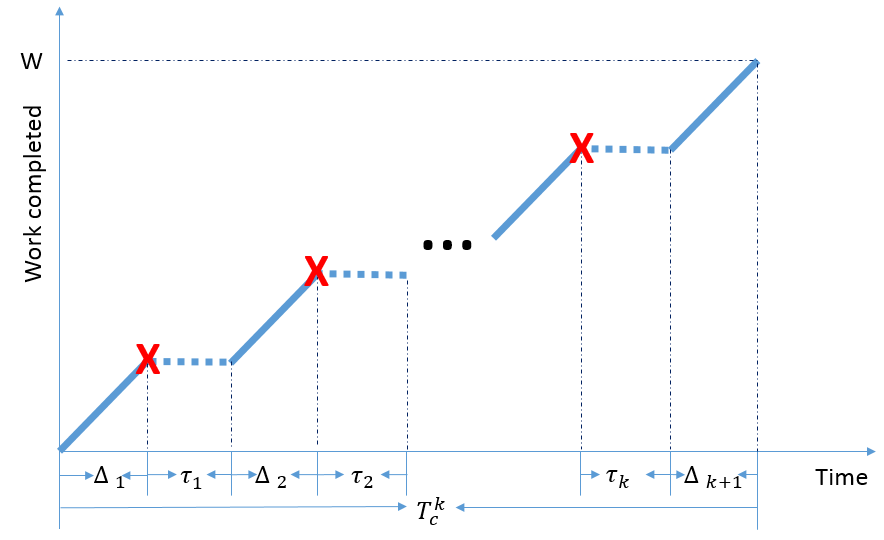
\includegraphics[width=0.7\columnwidth]{Figures/progress}
	\end{center}
	%\vskip -0.22in 
	\caption{Illustration of application's progress with failure incurred delays.}
	\label{fig:progress}
\end{figure}

Since Lazy Shadowing use $M$ cores for executing main processes and $S$ cores for shadowing ($M+S=N$), the total workload $W$ will be split into $M$ tasks, each of which will be assigned a pair of main and shadow processes. Therefore, the workload of each process is 
$w=W/M$. The following theorem gives the expression for the completion time, $T_c^k$, when there are $k$ failures.

\begin{theorem}
If no subsequent failure happens before the recovery of the previous failure, then using Lazy Shadowing, 
	$$T_c^k = w + (1-\sigma_s^b)\sum_{i=1}^k\Delta_i$$
\end{theorem}
%\begin{proof}
{\sc Proof}. The recovery time $\tau_i$ is the time needed for the lazy shadow of the failed main to catch up. Under Leaping Shadows, it is guaranteed that all the shadows reach the same execution point as the mains (See Figure~\ref{fig:leap}) after the previous recovery, so every recovery time is proportional to its previous continuous execution length, which is $\Delta_i$. That is, $\tau_i = \Delta_i \times (1 - \sigma_s^b)$ (The value of $\Delta_i$ can be obtained given a failure probability distribution, as will be demonstrated in Section~\ref{sec:evaluation}). The total delay induced by all $k$ failures is $\sum_{i=1}^k\tau_i$.
Since we assume there are $k$ failures, then $\Delta_{k+1}$ is the failure free execution interval until the workload is complete, i.e., $\Delta_{k+1} = w - \sum_{i=1}^{k}\Delta_i$. Finally, according to Figure~\ref{fig:progress}, the completion time with $k$ failures is 
	$T_c^k = \sum_{i=1}^{k+1}\Delta_i + \sum_{i=1}^k\tau_i = w + (1-\sigma_s^b)\sum_{i=1}^k\Delta_i$.
%\end{proof}
    $\square$

Although it may seem that the delay would keep deteriorating as the number of failures increases, 
it turns out to be well bounded, as a benefit of Leaping shadows:

\begin{corollary}
The delay induced by failures is bounded by $(1-\sigma_s^b)w$.
\end{corollary}
%\begin{proof}

{\sc Proof}. From above theorem we can see the delay from $k$ failures is $(1-\sigma_s^b)\sum_{i=1}^k\Delta_i$. It is straightforward that, for any non-negative integer of $k$, we have the equation $\sum_{i=1}^{k+1}\Delta_i= w$. As a result, 
$\sum_{i=1}^{k}\Delta_i = w - \Delta_{k+1} \le w$. Therefore, $(1-\sigma_s^b)\sum_{i=1}^k\Delta_i \le (1-\sigma_s^b)w$, which means the delay is bounded by $(1-\sigma_s^b)w$.
%\end{proof}
$\square$

Typically, the number of failures to be encountered will not be known before the execution. Given a failure distribution, however, we can estimate the probability for a specific value of $k$. We assume that failures do not occur during recovery, so the failure probability of a core during the execution can be estimated as $P_c = F(w)$. Then the probability that there are $k$ failures among the $N$ cores during the execution is 
\begin{equation}
\begin{split}
P_s^{k}= & \dbinom{N}{k}{P_c}^k(1-P_c)^{N-k} \\
%= & \dbinom{M}{k}({\frac{w}{MTTI}})^k(1-\frac{w}{MTTI})^{M-k}
\end{split}
\end{equation}

The following theorem gives an expression for the expected completion time, $T_{total}$, considering all possible cases of failures. 

\begin{theorem}
If no subsequent failure happens before the recovery of the previous failure, then using Lazy Shadowing,
$T_{total} = T_{c} / (1 - P_a)$, where $T_{c} = \sum_{i} T_{c}^{i} \cdot P_s^{i}$.
\end{theorem}
%\begin{proof}

{\sc Proof}. If application failure does not happen, the completion time considering all possible failures can be averaged as $T_{c} = \sum_{i} T_{c}^{i} \cdot P_s^{i}$. If application failure occurs, however, the application needs to restart from the beginning. Considering the possibility of re-execution, the total expected completion time is $T_{total} = T_{c} / (1 - P_a)$.
%\end{proof}
$\square$

Process replication is a special case of Lazy Shadowing where $\alpha=1$, so we can use the above theorem to derive the expected completion time for process replication:

\begin{corollary}
The expected completion time for process replication is $T_{total} = 2W/N / (1 - P_a)$.
\end{corollary}
%\begin{proof}

{\sc Proof}. Using process replication, half of the available cores are dedicated to replicas so that the workload assigned to each task is significantly increased given the fixed number of cores available, i.e., $w=2W/N$. Different from the case of $\alpha \ge 2$, failures do not incur any delay unless application failure occurs, since the replicas are executing at the same rate as the main processes. As a result, the completion time of process replication without application failure is constant with respect to the number of failures, i.e., $T_c^k=w=2W/N$. Therefore, the completion time, $T_c$, considering all values of $k$, is also $2W/N$. Finally, the expected completion time considering the possibility of re-execution is $T_{total} = T_c / (1 - P_a) = 2W/N / (1 - P_a)$.
%\end{proof}
$\square$

A closer look at the above analysis one can realize that Lazy Shadowing has both advantage and disadvantage compared to traditional process replication. When collocating multiple shadow processes on each core, more than half of the available cores will be dedicated to main processes, leading to less workload per process. At the same time, collocation slows down the shadow processes, which incurs delays when failures occur. We will discuss more about the conflicting effects in Section~\ref{sec:evaluation}.
 %Although it may seem that the delay would keep deteriorating as the number of failures increases, it turns out to be well bounded, as a result of shadow leaping. From Equation~\ref{eq:time_k} we can see the delay of $k$ failures is $(1-\sigma_s^b)\sum_{i=1}^k\Delta_i$. Since we have the relation $\Delta_{k+1} = w - \sum_{i=1}^{k}\Delta_i$, $\sum_{i=1}^{k}\Delta_i$ is bounded by $w$, effectively limiting the delay by $(1-\sigma_s^b)w$.

%Contrary to process replication and Lazy Shadowing, checkpointing can use all the available cores to share the total workload, so that $w = W/M$. However, the drawback is that each failure would result in an application failure which needs to roll back the execution to the last checkpoint. With that said, the recovery time of each failure is equal to the normal execution time from the last checkpoint to the time of the failure, i.e., $\tau_i = \sum_{j=1}^{i}\Delta_j$. The completion time with $k$ failures is $T_c^k = \sum_{i=1}^{k+1}\Delta_i + \sum_{i=1}^k\tau_i = w + \sum_{i=1}^{k}\sum_{j=1}^i\Delta_j$.

%\subsubsection{Expected energy consumption}







\subsection{Expected energy consumption}
\label{anal_energy}
The power consumption of one core consists of two parts, dynamic power, $p_d$, which exists only when the core is executing, and static power, $p_s$, which is constant as long as the machine is on. This can be modeled as $p = p_d + p_s$. Note that in addition to CPU leakage, other components, such as memory and disk, also contribute to static power. 

%For checkpointing and process replication, all cores are running all the time until the application is complete. Therefore, the energy consumption is proportional to the total execution time, and the expected energy consumption when using $M$ cores to execute an application is calculated as 
For process replication, all cores are running all the time until the application is complete. Therefore, the expected energy consumption, $En$, is proportional to the expected execution time $T_{total}$: 
\begin{equation}
%En = N * p * T_{total}
En = N \times p \times T_{total}
\label{eq:exp_energy1}
\end{equation} 
%Although the failed components should not consume any power, we ignore this since the number of failures is negligible compared to the total number of cores.

Lazy Shadowing has the potential to save power compared to process replication, since main cores are idle during the recovery time after each failure, and the shadows can achieve forward progress through shadow leaping. During the normal execution time, all the cores consume static power as well as dynamic power. During recovery time, however, the main cores are idle and consume only static power, while the shadow cores first perform shadow leaping and then become idle. Altogether, the expected energy consumption for Lazy Shadowing can be modeled as 
\begin{equation}
En = N \times p_s \times T_{total} + N \times p_d \times w + S \times p_{l} \times T_l.
%En = N * p_s * T_{total} + N * p_d * w + S * p_{l} * T_l.
\label{eq:exp_energy2}
\end{equation}
with $p_{l}$ denoting the dynamic power consumption of each core during shadow leaping and $T_l$ the expected total time spent on leaping. %Based on Equation~\ref{eq:exp_energy2} and Corollary 1.1, we can also establish an upper bound on the expected energy consumption for Lazy Shadowing:

%\begin{theorem}
%If no subsequent failure happens before the recovery of the previous failure, then using Lazy Shadowing, the upper bound on expected energy consumption is
%$(2N * p_s + N * p_d + S * p_{l})*w$.
%\end{theorem}
%\begin{IEEEproof}
%From Corollary 1.1 we know that the delay is at most $(1-\sigma_s^b)w \le w$, so $T_{total} \le 2w$. Also, since the leaping time overlaps with the recovery time (delay), $T_l \le (1-\sigma_s^b)w \le w$. Therefore, $En = N * p_s * T_{total} + N * p_d * w + S * p_{l} * T_l \le N * p_s * (2w) + N * p_d * w + S * p_{l} * w = (2N * p_s + N * p_d + S * p_{l})*w$.
%\end{IEEEproof}

